\section{The structure of the groups}\label{sec:group-structure}

This section asks what holds the groups of Section~\ref{sec:structure} together, what shape they
take, who leads them, with whom pilots fly, and where the distribution of sizes comes from. Chance
is again the null model of Section~\ref{sec:null}. The graph terms used here (shape, order,
configuration model) are defined in Appendix~\ref{app:graphs}, the two models in
Appendix~\ref{app:models}. Some results refer to the report \emph{Group and solo flights}
(\texttt{analysis/groups/group-identification}), which compares the motion of pilots in a group
and alone.

\subsection{Cohesion: what keeps two pilots together}\label{sec:cohesion}

Inside a contact, the delay $\ell^*(t)$ of Section~\ref{sec:lag} says how many seconds one pilot is
behind the other on the same path; instants with either pilot in a search are left out. Groups: the
\StCohReal{} pair intervals of pilots who took off within 10~km. Chance: the \StCohChance{} contacts
of the surrogate pairs, two pilots who never saw each other; the \StCohChanceLong{} that last at
least $\tau^*$ are selected as the groups are, by staying in contact that long.
\begin{itemize}
  \item $D(s)=\langle(\ell(t+s)-\ell(t))^2\rangle$, the mean square change of the delay after $s$,
        fitted by an Ornstein--Uhlenbeck process, $D(s)=2\sigma^2(1-e^{-ks})+c$: $1/k$ is how long
        the delay remembers its value, $\sigma$ its spread, $2k\sigma^2$ how fast it wanders.
  \item The drift $\langle\ell(t+60~\mathrm{s})-\ell(t)\rangle/60~\mathrm{s}$ at each $\ell$, made
        symmetric since the order of a pair is arbitrary: the pull back to $\ell=0$, a spring $-k\ell$
        near 0.
  \item The distance between the two pilots at the same instant after their first contact.
\end{itemize}
Two independent pilots separate as twice the displacement variance of one, not twice its MSD: they
share the drift along the route. The surrogate pairs give this baseline directly, with the same
terrain.

\begin{figure}
\centering
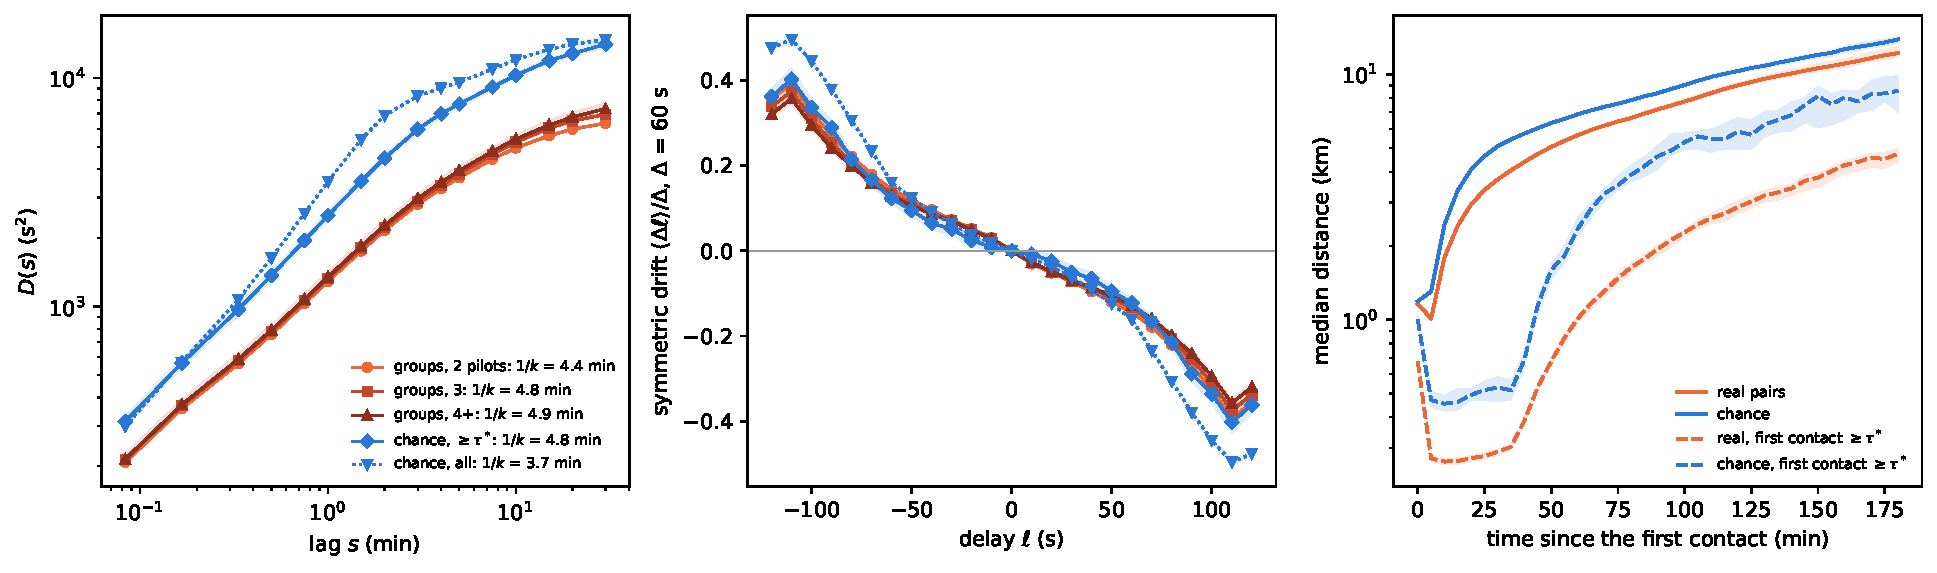
\includegraphics[width=\textwidth]{figures/structure/cohesion.pdf}
\caption{Left: $D(s)$ of groups (by size) and of chance contacts, with $1/k$ of the
Ornstein--Uhlenbeck fit. Middle: symmetric drift of the delay. Right: median distance at the same
instant after the first contact, for every pair and for those whose first contact lasts at least
$\tau^*$. Bands: 5--95\% of 200 draws of the dates.}
\label{fig:cohesion}
\end{figure}

\begin{itemize}
  \item \textbf{Groups keep the same pace.} Their delay wanders at $2k\sigma^2=\StQReal$ \StQRealBand~s$^2$/s,
        against \StQChanceLong{} \StQChanceLongBand{} for chance contacts as long and \StQChance{}
        \StQChanceBand{} for all of them; its spread is $\sigma=\StSigmaReal$~s \StSigmaRealBand, against
        \StSigmaChance~s \StSigmaChanceBand.
  \item \textbf{They are not pulled back much harder.} The delay forgets itself in $1/k=\StOuReal$~min
        \StOuRealBand, against \StOuChance~min \StOuChanceBand{} by chance; the drift gives \StDriftReal~min
        \StDriftRealBand{} against \StDriftChance~min \StDriftChanceBand. Most of the pull is the
        selection: a contact that lasts keeps $|\ell|\le\delta$ by definition.
  \item \textbf{Size does not matter:} $2k\sigma^2=\StQTwo$, \StQThree{} and \StQFour~s$^2$/s at 2, 3 and 4+
        pilots.
  \item \textbf{They stay together after the contact that selected them.} When the first contact lasts
        at least $\tau^*$, the two pilots are \StSepRealLongSixty~km apart 60~min later (median), against
        \StSepChanceLongSixty~km by chance; \StSepRealLongTwoHours{} against \StSepChanceLongTwoHours~km
        after 2~h. Over every first contact, \StSepRealThirty{} against \StSepChanceThirty~km after 30~min.
\end{itemize}
A group is two pilots who keep the same pace, not two pilots tied by a spring. Whether this is
following or the same choices in the same air, the data cannot tell.

\subsection{Shape: chains or compact groups}\label{sec:chains}

Inside a configuration the members are fixed, but the pair intervals among them start and end.
Between two such changes the graph has a \emph{density} (the share of the member pairs in contact)
and a \emph{diameter} (the most steps between two members); its shape is \emph{complete} (every
member in contact with every other), a \emph{tree} (the fewest edges that keep the members
connected: a chain or a star) or between. The TA-MSD pieces of the report \emph{Group and solo
flights} lie inside one configuration and take the shape of the graph at their middle.

\begin{figure}
\centering
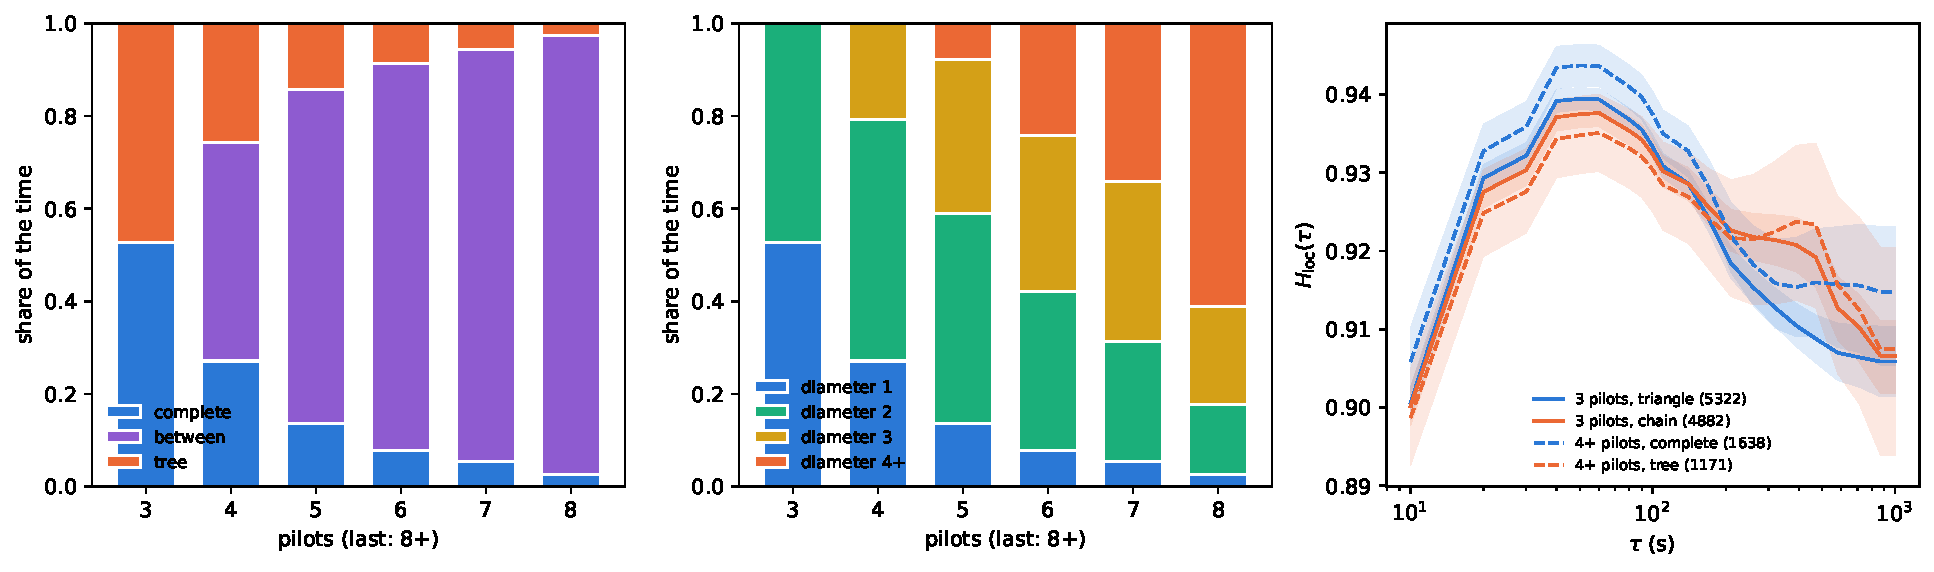
\includegraphics[width=\textwidth]{figures/structure/chains.pdf}
\caption{Left: share of the time of each shape, by size (8+ pooled). Middle: share of the time by
diameter. Right: $H_\mathrm{loc}(\tau)$ of paragliders in triangles and chains of 3 pilots, and in
complete and tree graphs of 4 or more (flights in brackets), with 5--95\% bands.}
\label{fig:chains}
\end{figure}

\begin{itemize}
  \item \textbf{Large groups are strings, not clouds.} Three pilots form a triangle \StTriangleThree\%
        of the time and a chain \StChainThree\%. Complete graphs fall from \StCompleteFour\% of the time
        at 4 pilots to \StCompleteMax\% at 8+, the mean density from \StDensityThree{} at 3 to
        \StDensityMax{} at 8+; at 8+ the diameter is 4 or more \StDiamFourMax\% of the time: pilots
        follow each other along the route.
  \item \textbf{The shape does not change the flight.} $H_\mathrm{loc}(1000~\mathrm{s})$ is
        \StHlocTriangle{} in triangles and \StHlocChain{} in chains; \StHlocComplete{} in complete graphs
        of 4+ and \StHlocTree{} in trees. The straighter progress found in \emph{Group and solo flights}
        does not need every pilot in contact with every other.
\end{itemize}

\subsection{Who leads}\label{sec:leaders}

The signed median delay $\ell_{\rm med}$ of a pair interval (Section~\ref{sec:lag}) says who passes
first: the pilot ahead, when the other passes at least 15~s later; otherwise the two fly abreast
(\Abreast\% of the pairs of two; median delay \DelayMedian~s). How leading changes the flight is in
\emph{Group and solo flights}. Here:
\begin{itemize}
  \item \textbf{order} in configurations of 3 pilots or more: each edge points from the pilot ahead
        to the one behind, a directed graph, against the same graphs with each direction drawn at
        random (50 draws);
  \item \textbf{switches} of the pilot ahead along $\ell^*(t)$ in the pair intervals of
        Section~\ref{sec:cohesion} (stretches shorter than 60~s dropped), against chance contacts
        lasting at least $\tau^*$;
  \item \textbf{who leads} in configurations of two named pilots: earlier flights in the catalog and
        wing class (A~=~1 to competition~=~5);
  \item \textbf{habitual leaders:} for the \HabitualPilots{} pilots with at least 10 roles in pairs, the
        dispersion of their lead fractions, against roles swapped at random.
\end{itemize}

\begin{figure}
\centering
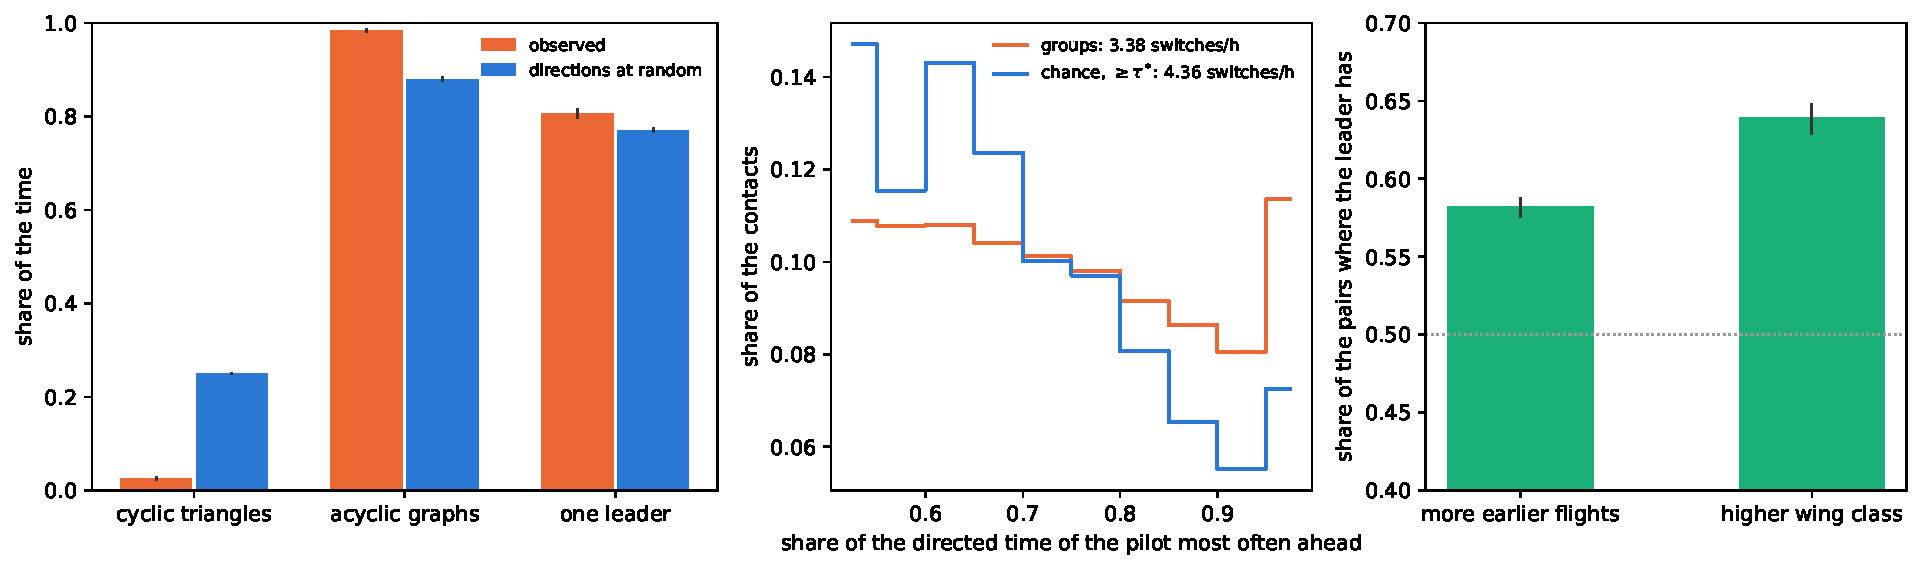
\includegraphics[width=\textwidth]{figures/structure/hierarchy.pdf}
\caption{Left: in groups of 3 or more, share of the time with cyclic directed triangles, acyclic
graphs (every edge directed) and one leader (acyclic graphs), observed and with directions at
random. Middle: share of the directed time of the pilot most often ahead in each contact, with the
switches per hour. Right: share of the pairs of two in which the leader has more earlier flights,
or the higher wing class. Bars: 5--95\% (blocks).}
\label{fig:hierarchy}
\end{figure}

\begin{figure}
\centering
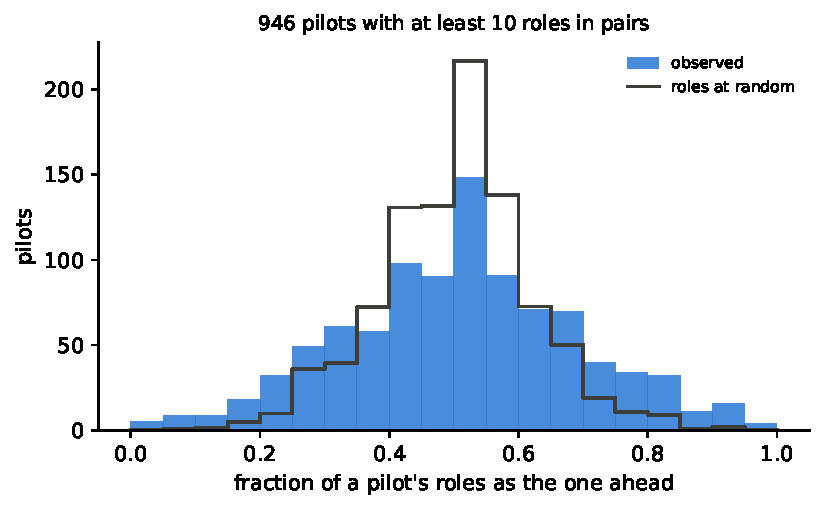
\includegraphics[width=0.48\textwidth]{figures/structure/mechanisms_habitual.pdf}
\caption{Lead fraction of each pilot, against roles at random.}
\label{fig:habitual}
\end{figure}

\begin{itemize}
  \item \textbf{Pilots are in a line.} Directed triangles are cyclic \StCyclic\% \StCyclicBand{} of the
        time, against \StCyclicNull\% at random; graphs with every edge directed (\StFullShare\% of the
        time) are acyclic \StAcyclic\%, against \StAcyclicNull\%. Positions along one route cannot form
        cycles: this is geometry, not rank.
  \item \textbf{One leader, in small groups:} \StOneLeader\% \StOneLeaderBand{} of the acyclic time,
        against \StOneLeaderNull\% \StOneLeaderNullBand{} at random; \StOneLeaderThree\% at 3 pilots,
        \StOneLeaderFour\% at 4, \StOneLeaderFive\% at 5 or more. A single file (depth $n-1$):
        \StLineThree, \StLineFour{} and \StLineFive\%.
  \item \textbf{The lead changes often.} The pilot ahead changes \StSwitches{} times per hour of contact
        \StSwitchesBand{}, against \StSwitchesChance{} \StSwitchesChanceBand{} by chance; the pilot most
        often ahead holds \StDominant\% of the directed time (median), against \StDominantChance\%.
  \item \textbf{The experienced pilot on the faster wing leads.} The leader has more earlier flights in
        \StExp\% \StExpBand{} of \StExpPairs{} pairs (\StExpRatio{} times as many, median), the higher
        wing class in \StWing\% \StWingBand{} of \StWingPairs.
  \item \textbf{Some pilots lead or follow persistently:} dispersion of the lead fractions
        \HabitualDispersion{} against \HabitualNull{} at random (95\% below \HabitualNullHigh);
        \HabitualExtreme\% lead in at most 20\% or at least 80\% of their roles, against
        \HabitualExtremeNull\% expected.
\end{itemize}

\subsection{Repeated partners}\label{sec:partners}

Paraglider pilots by their name in the catalog (anonymised ones left out). Two pilots are partners
on a day when their flights share a pair interval: a \emph{pair-day}. Chance keeps who flies in a
group where and when: within each site-day (takeoffs within 3~km, joined when a pair interval links
two sites), the partners are redrawn at random, each pilot keeping its number of partners that day
(a configuration model; 100 draws).

\begin{figure}
\centering
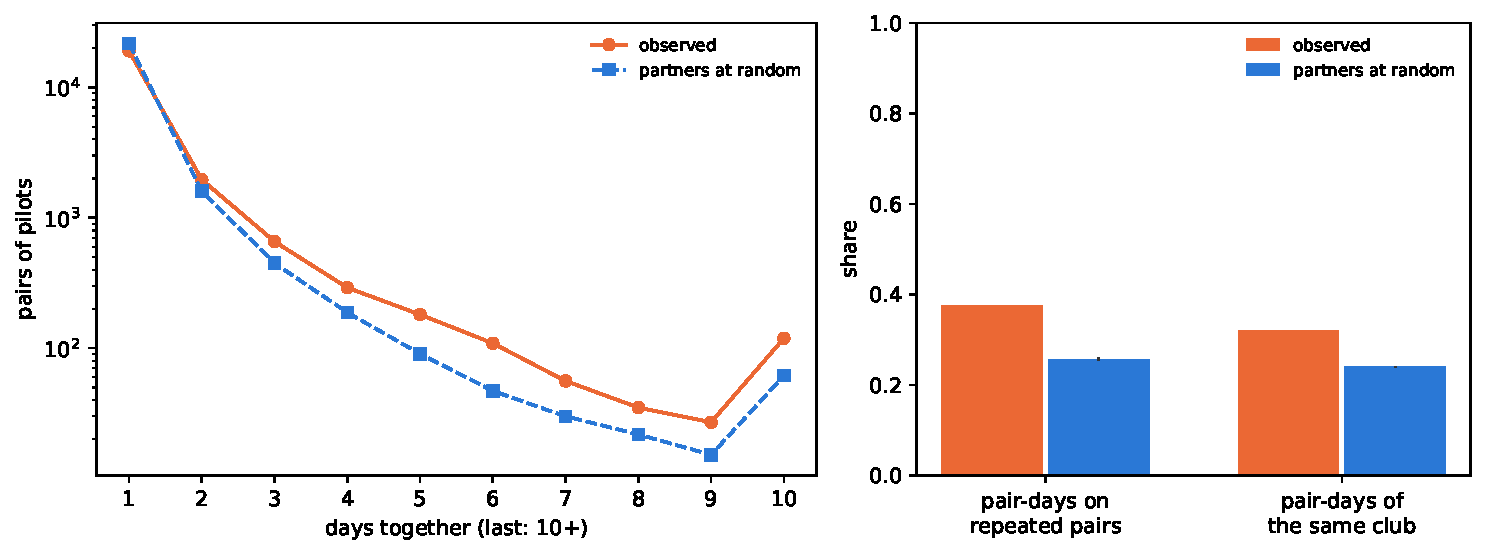
\includegraphics[width=0.85\textwidth]{figures/structure/partners.pdf}
\caption{Left: pairs of pilots by the number of days they flew together, observed and with
partners at random. Right: share of the pair-days on pairs that meet on more than one day, and of
two pilots of the same club (each pilot's main club); bars at random: 5--95\% of the draws.}
\label{fig:partners}
\end{figure}

There are \StPairDays{} pair-days among \StPilots{} pilots and \StPairs{} pairs; one pair flew
together on \StMaxDays{} days.
\begin{itemize}
  \item \textbf{Pilots return to the same partners:} \StRepeatObs\% of the pair-days are on pairs
        that meet on more than one day, against \StRepeatNull\% \StRepeatNullBand{} at random
        (\StRepeatPairsObs{} such pairs against \StRepeatPairsNull).
  \item \textbf{and to their club:} \StSameClubObs\% of the pair-days join two pilots of the same
        club, against \StSameClubNull\% \StSameClubNullBand.
\end{itemize}
Chance already fixes who flies in a group at each site and day, so the excess is the choice of
partner among the pilots there. Choosing where and when to fly with friends is not removed: it is
part of chance here.

\subsection{Fission and fusion: where the sizes come from}\label{sec:fission}

$T(n)$ is the share of the time spent in configurations of $n$ pilots: the chance that a group seen
at a random instant has $n$ pilots. If sizes change one pilot at a time, the flux from $n$ to $n+1$
pilots balances the flux back, a birth--death chain:
\begin{equation}\label{eq:chain}
  \frac{T(n+1)}{T(n)}=\frac{g(n)}{l(n+1)},
\end{equation}
with $g(n)$ the joins and $l(n)$ the leaves and landings per hour at size $n$
(Table~\ref{tab:rates}). Splits and merges are left out. Per member, $g(n)=a\,n$ and
$l(n)=\mu\,n^{1-\gamma}$: every member brings in others at rate $a$ and leaves at rate
$\mu n^{-\gamma}$, fitted to the rates, not to $T$. With $\gamma=0$ the chain gives the log-series
$T(n)\propto x^n/n$, $x=a/\mu$. For comparison, the form of Bonabeau et al.~\cite{bonabeau1999},
$T(n)\propto n^{-\alpha}e^{-n/n_c}$, fitted to $T$.

\begin{figure}
\centering
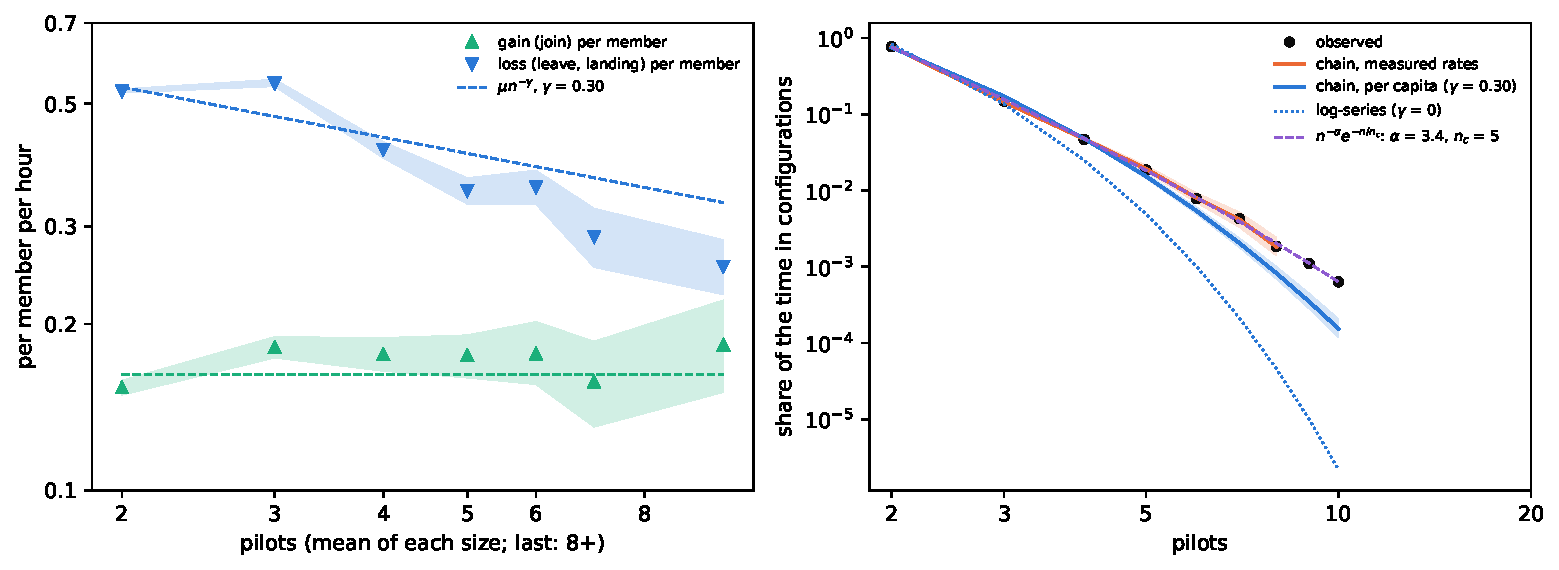
\includegraphics[width=0.9\textwidth]{figures/structure/fission.pdf}
\caption{Left: joins and losses per member per hour by size (mean size of each class; 8+ pooled),
with $a$ and $\mu n^{-\gamma}$ dashed. Right: $T(n)$ observed (sizes with at least 10~h) and from
the chain~\eqref{eq:chain} with the measured rates, with the per-capita rates and with $\gamma=0$;
dashed purple: the form of Bonabeau et al.\ fitted to $T$. Bands: 5--95\%.}
\label{fig:fission}
\end{figure}

\begin{itemize}
  \item \textbf{One pilot at a time is enough.} With the measured rates the chain gives $T(n)$ within
        4\% from 2 to 8 pilots (\StChainThreePred{} against \StChainThreeObs{} at 3 pilots, just outside
        its band), although splits and merges are \StMultiTwo\% of the changes at 2 pilots and
        \StMultiMax\% at 8+.
  \item \textbf{Joining grows with the members, leaving does not.} Each member brings in others at
        $a=\StCapitaA$ \StCapitaABand{} per hour, at every size. Each leaves at \StLossTwo{} per hour in a
        pair and \StLossMax{} at 8+: $\gamma=\StGamma$ \StGammaBand.
  \item \textbf{The heavy tail comes from staying.} With $\gamma=0$ ($x=\StX$) $T(\StNTop)$ is
        \StLogSeriesFactor{} times too small; with $\gamma=\StGamma$, \StCapitaFactor{} times. Fitted
        directly, $\alpha=\StAlpha$ and $n_c=\StNc$.
\end{itemize}

\subsection{What the structure says}\label{sec:conclusions}

\noindent
\begin{minipage}[t]{0.49\textwidth}
\textbf{Supported}
\begin{itemize}
  \item groups are mostly pairs; large ones are strings along the route that change members every
        few minutes, while the episode lasts about an hour;
  \item group pilots keep the same pace: their delay wanders half as fast as that of two pilots
        kept in contact by chance, and they stay closer after the contact;
  \item the size distribution follows from one pilot joining or leaving at a time; its heavy tail
        from members of larger groups leaving less often;
  \item the lead changes a few times per hour and goes more often to the experienced pilot on the
        higher wing;
  \item pilots return to the same partners and to their club mates more than who flies where and
        when explains.
\end{itemize}
\end{minipage}\hfill
\begin{minipage}[t]{0.49\textwidth}
\textbf{Not supported}
\begin{itemize}
  \item a spring that pulls pilots back: the pull is about that of chance contacts selected the
        same way;
  \item that the shape of a group (triangle or chain, complete or tree) changes how its pilots fly;
  \item a social rank from the order in a group: a line along the route is geometry;
  \item that keeping pace means following: the surrogate pairs fly at another hour, so pilots in
        the same air at the same time may share the pace without seeing each other;
  \item pilots are names of the catalog: homonyms join, a pilot who changes name splits.
\end{itemize}
\end{minipage}

\medskip
The delay $\ell^*(t)$ that the cohesion and the switches of the lead read instant by instant is
undetermined in a thermal within the window that altitude allows (Section~\ref{sec:lag}), for real
and chance contacts alike: the comparisons with chance carry this noise on both sides.
